\documentclass[12pt,a4paper]{report}
\usepackage[utf8]{inputenc}
\usepackage[margin=0.7in]{geometry}
\usepackage{graphicx}
\usepackage{tabularx}
\usepackage{booktabs}
\usepackage{float}
\usepackage{xltabular}
\usepackage{enumitem}
\usepackage{times}
\usepackage{titlesec}
\usepackage{listings}
\usepackage{xcolor}
\usepackage{hyperref}
\usepackage{tocloft}
\usepackage{indentfirst}
\usepackage{caption}
\usepackage{mdframed}


\definecolor{termbg}{RGB}{30, 30, 30} 
\definecolor{termfg}{RGB}{230, 230, 230}
\definecolor{termgreen}{RGB}{80, 250, 123}
\definecolor{termblue}{RGB}{139, 233, 253}
\lstdefinestyle{terminal}{
    backgroundcolor=\color{termbg},
    basicstyle=\color{termfg}\ttfamily\small,
    keywordstyle=\color{black},              
    commentstyle=\color{gray}\itshape,
    stringstyle=\color{red},
    frame=single,        
    frameround=tttt,      
    rulecolor=\color{termbg!80!black},     
    framesep=8pt,            
    xleftmargin=8pt,                      
    xrightmargin=8pt,                       
    breaklines=true,                    
    showstringspaces=false,                  
    literate={\$}{{\textcolor{termgreen}{\$}}}1 
}

\lstset{style=terminal}

\newmdenv[
  topline=false,
  bottomline=false,
  rightline=false,
  leftline=true,
  linewidth=3pt,
  linecolor=gray,
  backgroundcolor=gray!10,
  innerleftmargin=10pt,
  innerrightmargin=10pt,
  innertopmargin=8pt,
  innerbottommargin=8pt
]{markdownnote}

\hypersetup{
    colorlinks=true,
    linkcolor=black,
    urlcolor=blue,
}

\lstset{
    basicstyle=\ttfamily\small,
    backgroundcolor=\color{gray!10},
    frame=single,
    breaklines=true,
    showstringspaces=false,
    columns=flexible,
    keepspaces=true,
}

\titleformat{\chapter}[display]
  {\normalfont\huge\bfseries\centering} 
  {\chaptertitlename\ \thechapter}
  {20pt}
  {\Huge}
\titlespacing*{\chapter}{0pt}{10pt}{40pt}

\begin{document}

\begin{titlepage}
    \centering
    \vspace*{1cm} 

    {\Large \textbf{UNIVERSITY OF COMPUTER STUDIES, YANGON}} \\[0.4cm]
    {\large Faculty of Computer Systems and Technologies} \\[0.2cm]
    {\large 2025 - 2026 Academic Year} \\[1.5cm]
   
    
\includegraphics[width=0.2\textwidth]{../src/ucsy-logo.png} \\[1.5cm]

    {\large \textbf{Linux Fundamentals (CST-311)}} \\[0.5cm]
    {\LARGE \textbf{Web Server}} \\[0.5cm]
    {\large Supervised by Daw Cho Cherry Aung} \\[2.5cm]

    {\large Submitted By} \\[0.8cm]
    {\large
    \begin{tabular}{l l}
		Mg Maung Khant & YKPT - 22988\\
		Mg Aung Myint Myat Aung & YKPT - 23029\\
		Mg Gon Yaung Win & YKPT - 23013\\
		Mg Aung Khant Kyaw & YKPT - 23023\\
		Ma San Thiri Tun & YKPT - 23078\\
		Mg Kaung Htut Thaw & YKPT - 23020\\
		Mg Han Linn Htun & YKPT - 23005\\
		Ma Shoon Lae Aung & YKPT - 23026\\
		Mg Aung Myint Myat & YKPT - 23046\\
    \end{tabular}
    }

    \vfill
    \noindent
    {\large September, 2026} \hfill 
    \begin{tabular}{r}
        {\large Semester IV} \\
        {\large B.C.Sc/B.C.Tech}
    \end{tabular}
\end{titlepage}
\newpage
\tableofcontents
\thispagestyle{empty}
\clearpage
\newpage

\thispagestyle{empty}
\newpage
\begin{center}
    {\huge \textbf{Abstract}}
\end{center}
\vspace{1em}

\indent This project presents the design, deployment, and hardening of a secure web server on a VMware virtual machine running Ubuntu 24.04 LTS. An Apache2 reverse proxy fronts a self-placed course website (the ``lfs-101-notes'' Next.js application), with TLS termination via a self-signed certificate and automatic HTTP-to-HTTPS redirection. The server is managed through Linux system administration best practices: dedicated user and group accounts (sysadmin for administration, dev for deployment), least-privilege file ownership, key-only SSH authentication, a UFW firewall restricting access to SSH (22), HTTP (80), and HTTPS (443), and fail2ban intrusion prevention. Tailscale provides a secure WireGuard-based tunnel for remote administration. The deployment process is automated by a Bash script that handles system updates, user creation, Apache2 configuration, Node.js and PM2 installation, and application deployment. All configuration is version-controlled and documented, demonstrating the practical application of Linux system administration concepts in a real-world scenario.

\vfill
\clearpage
\newpage

\pagenumbering{arabic}
\setcounter{page}{1}

\chapter{Introduction}
\section{Introduction}

\indent Linux system administration is a core skill in modern IT infrastructure. This project applies lecture concepts from the Linux Fundamentals course (CST-311) to a real-world scenario: deploying and securing a web server on a VMware virtual machine.

The project sets up an Apache2 web server hosting a Next.js application---a self-paced course website---on Ubuntu 24.04 LTS. Rather than simply running a default server, the team implements proper Linux administration practices including user and group management, file permission enforcement, service hardening, firewall configuration, and intrusion prevention.

The resulting system follows the principle of least privilege: the web server process, the deployment user, and the administrative accounts each have only the permissions they need---no more. Production traffic reaches the site directly via the VM's IP address, while administrative access is routed through an encrypted Tailscale tunnel.

\section{Project Objectives}

The objectives of this project are:

\begin{enumerate}[leftmargin=2em]
    \item Deploy a Next.js application on a VMware virtual machine running Ubuntu 24.04 LTS, accessible via a web browser on the network.
    \item Configure Apache2 as a reverse proxy with TLS termination, serving the application on HTTPS.
    \item Apply Linux user and group management to enforce least-privilege access for administration and deployment.
    \item Implement file permission controls so the web server cannot modify its own document root.
    \item Harden SSH with key-only authentication and disable root login.
    \item Configure a UFW firewall allowing only SSH (22), HTTP (80), and HTTPS (443).
    \item Deploy fail2ban to automatically ban IPs after repeated failed login attempts.
    \item Use Tailscale for secure remote administration via a WireGuard tunnel.
    \item Automate the deployment process with a Bash script for reproducibility.
\end{enumerate}

\newpage

\chapter{Background Theory}
\section{Operating System}

\indent An operating system (OS) is system software that manages computer hardware and software resources and provides common services for computer programs. It acts as an intermediary between users and the computer hardware, handling memory management, process scheduling, file system management, and device I/O.

\begin{figure}[h]
    \centering
    \fbox{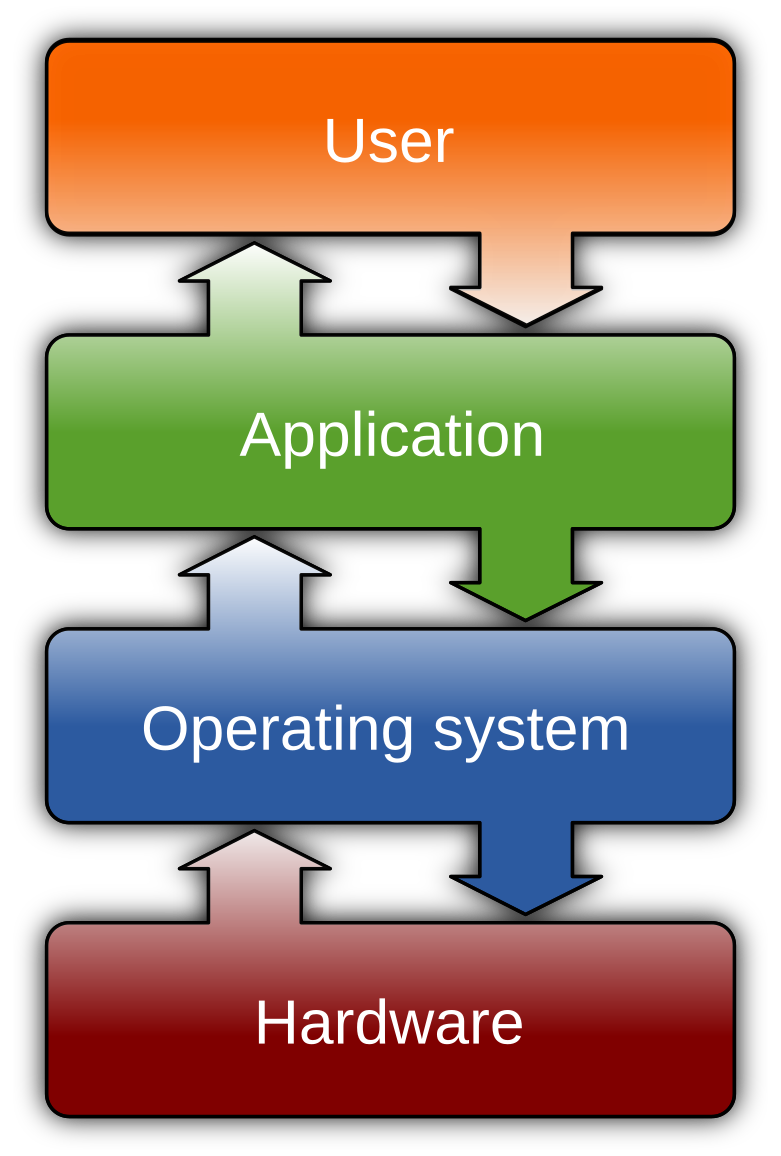
\includegraphics[width=0.25\textwidth]{../src/os.png}}
    \caption{Operating System \texttt{//Source:WiKi}}
\end{figure}

The operating system can be divided into several layers: the kernel (which interacts directly with hardware), system libraries (which provide APIs for applications), and the user interface (which allows human interaction). In server environments, reliability, security, and performance are the primary concerns, making Unix-like operating systems - particularly Linux - the dominant choice for web infrastructure.

\begin{figure}[h]
    \centering
    \fbox{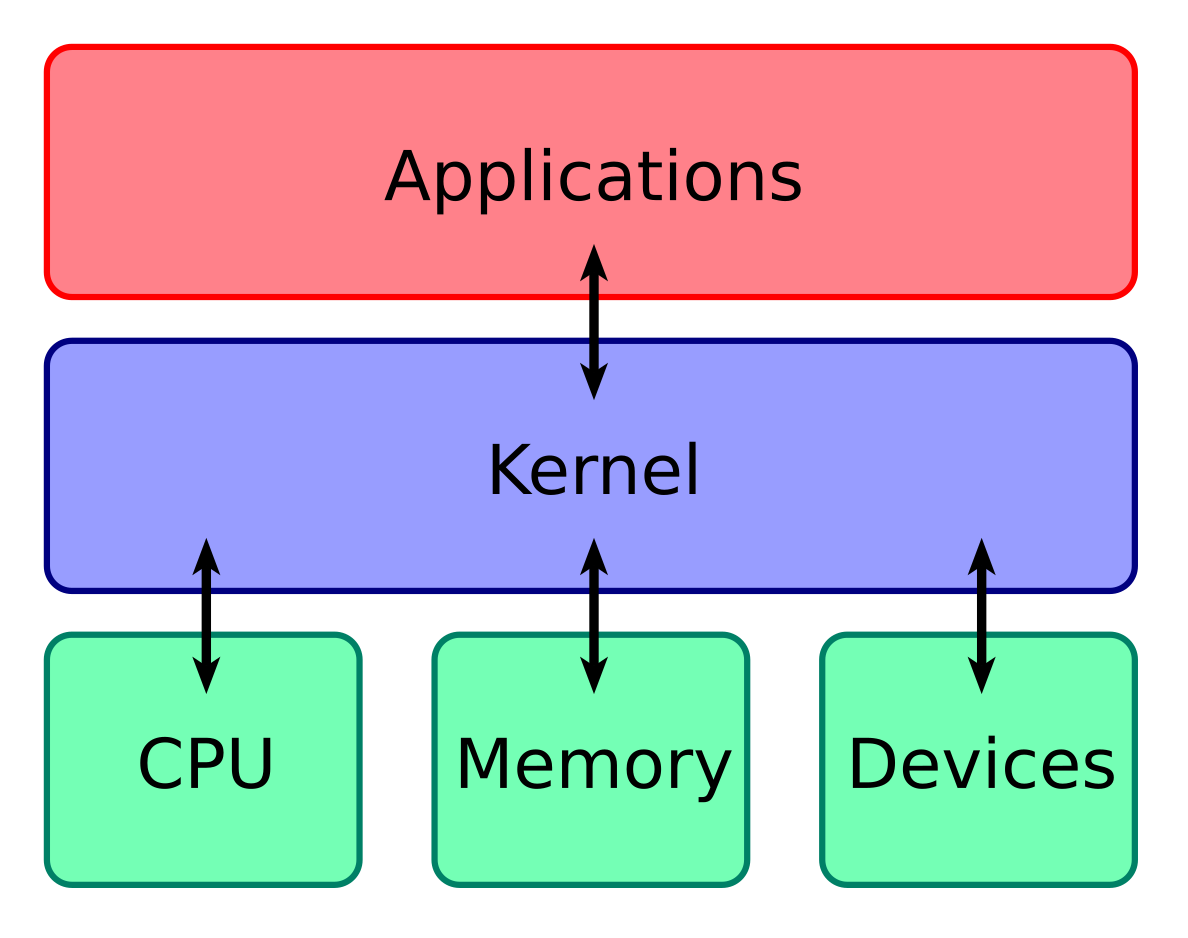
\includegraphics[width=0.25\textwidth]{../src/kernel.png}}
    \caption{Kernel \texttt{//Source:WiKi}}
\end{figure}

\section{Linux Distribution}

\indent A Linux distribution (distro) is an operating system built on the Linux kernel, bundled with system libraries, package managers, and application software. Each distribution targets a specific use case and provides its own package management system, release cycle, and default configuration.

Common distributions include:

\begin{itemize}[leftmargin=2em]
    \item \textbf{Ubuntu} --- Debian-based, widely used for servers and cloud infrastructure. Uses the \texttt{apt} package manager and releases LTS (Long Term Support) versions every two years.
    \item \textbf{CentOS / Rocky Linux} --- RHEL-based, popular in enterprise environments. Uses \texttt{yum} / \texttt{dnf}.
    \item \textbf{Debian} --- Known for stability; Ubuntu is derived from it.
    \item \textbf{Fedora} --- Cutting-edge features, often previewing what enters RHEL.
\end{itemize}

\begin{figure}[h]
    \centering
    \fbox{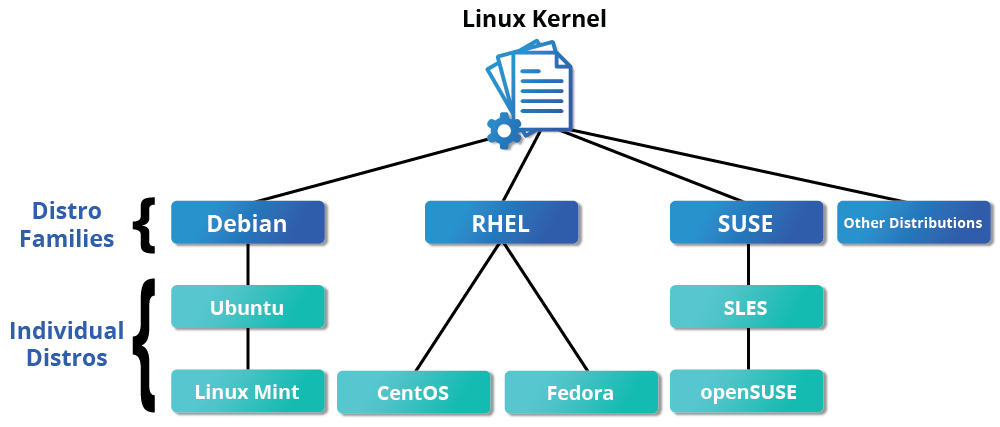
\includegraphics[width=0.9\textwidth]{../src/distro.png}}
    \caption{Linux Distro \texttt{//Source:Linux Foundation}}
\end{figure}

This project uses \textbf{Ubuntu 24.04 LTS} (Noble Numbat) because of its five-year support window, extensive documentation, and large community. The LTS designation means security patches and bug fixes are guaranteed until April 2029, making it suitable for production server deployments.

\section{GUI and CLI}

\indent A \textbf{Graphical User Interface (GUI)} allows users to interact with the system through windows, icons, and visual elements. While intuitive for desktop use, GUIs consume additional resources and are impractical for remote server management.

A \textbf{Command-Line Interface (CLI)} allows users to interact with the system by typing commands in a terminal. For server administration, the CLI is preferred because:

\begin{itemize}[leftmargin=2em]
    \item It consumes minimal system resources.
    \item Commands can be scripted and automated.
    \item Remote access over SSH works efficiently even on low-bandwidth connections.
    \item System configuration files are text-based and can be edited directly.
\end{itemize}

\begin{figure}[h]
    \centering
    \fbox{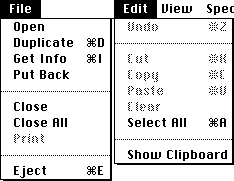
\includegraphics[width=0.5\textwidth]{../src/gui.png}}
    \caption{GUI \texttt{//Source:WiKi}}
\end{figure}

\begin{figure}[h]
    \centering
    \fbox{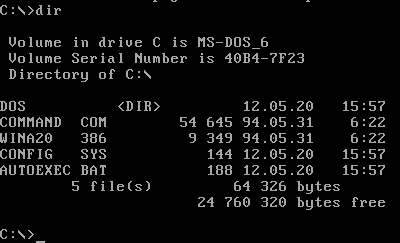
\includegraphics[width=0.5\textwidth]{../src/cli.png}}
    \caption{CLI \texttt{//Source:WiKi}}
\end{figure}

All configuration in this project is performed via the CLI using tools such as \texttt{bash}, \texttt{nano}, \texttt{ssh}, and \texttt{systemctl}. The server runs without a desktop environment.

\section{Different Types of Linux Server}

\indent Linux servers are classified by the services they provide:

\begin{itemize}[leftmargin=2em]
    \item \textbf{Web Server} --- Serves HTTP/HTTPS content to clients. Common software: Apache2, Nginx.
    \item \textbf{Database Server} --- Stores and retrieves structured data. Common software: MySQL, PostgreSQL.
    \item \textbf{File Server} --- Provides shared file storage over a network. Common software: Samba, NFS.
    \item \textbf{Mail Server} --- Handles email sending and receiving. Common software: Postfix, Dovecot.
    \item \textbf{DNS Server} --- Resolves domain names to IP addresses. Common software: BIND9.
    \item \textbf{DHCP Server} --- Automatically assigns IP addresses to network devices. Common software: ISC DHCP.
    \item \textbf{Proxy Server} --- Intermediary for client requests, providing caching and access control. Common software: Squid.
    \item \textbf{VPN Server} --- Provides encrypted remote access. Common software: WireGuard, OpenVPN.
\end{itemize}

This project implements a \textbf{web server} using Apache2 as the primary service, with Node.js and PM2 serving a Next.js application on the backend.

\newpage

\chapter{Implementation}

\section{Installation Operating System}

\indent Ubuntu 24.04 LTS (Noble Numbat) was installed on a VMware Workstation virtual machine with the following allocated resources:

\begin{table}[H]
\centering
\begin{tabular}{l l}
\toprule
\textbf{Resource} & \textbf{Allocation} \\
\midrule
CPU    & 2+ cores \\
RAM    & 4 GB minimum\\
Disk   & 40 GB+\\
Network & NAT \\
\bottomrule
\end{tabular}
\caption{Virtual machine resource allocation}
\end{table}

The installation process involved downloading the Ubuntu 24.04 LTS ISO, creating a new virtual machine in VMware Workstation, mounting the ISO, and completing the guided installation. A regular user account was created during installation for initial access.

\section{Ubuntu Operation System}

\indent Ubuntu 24.04 LTS was chosen for the following reasons:

\begin{itemize}[leftmargin=2em]
    \item \textbf{Long-term support:} Five years of security updates (until April 2029).
    \item \textbf{Community and documentation:} Extensive official guides and community forums.
    \item \textbf{Package availability:} The \texttt{apt} package manager provides all required software (Apache2, Node.js, UFW, fail2ban).
    \item \textbf{Cloud-init integration:} Works seamlessly with VMware's cloud-init for network configuration.
\end{itemize}

The server runs a minimal installation without a desktop environment, maximizing available resources for the web server and application.
\newpage

\section{System Requirements}

\indent The following packages and tools were installed on the server:

\begin{table}[H]
\centering
\small
\begin{tabularx}{\textwidth}{l X}
\toprule
\textbf{Component} & \textbf{Purpose} \\
\midrule
Apache2      & Web server and reverse proxy \\
Node.js (LTS) & Runtime for the Next.js application \\
npm          & Package manager for Node.js dependencies \\
PM2          & Process manager for Node.js (auto-restart, boot persistence) \\
certbot      & SSL/TLS certificate management (optional for domains) \\
UFW          & Firewall (Uncomplicated Firewall) \\
fail2ban     & Intrusion prevention (auto-bans repeated failed attempts) \\
OpenSSH      & Secure remote access (key-only authentication) \\
Tailscale    & WireGuard-based VPN for administrative access \\
\bottomrule
\end{tabularx}
\caption{Server software components}
\end{table}

\section{Ubuntu with VMware}
\begin{enumerate}
 \item Open VMware Workstation or Fusion on your machine.
 \item Click on “Create a New Virtual Machine”.
 \item Continue to create A Virtual Ubuntu Operating.

\begin{figure}[h]
    \centering
    \fbox{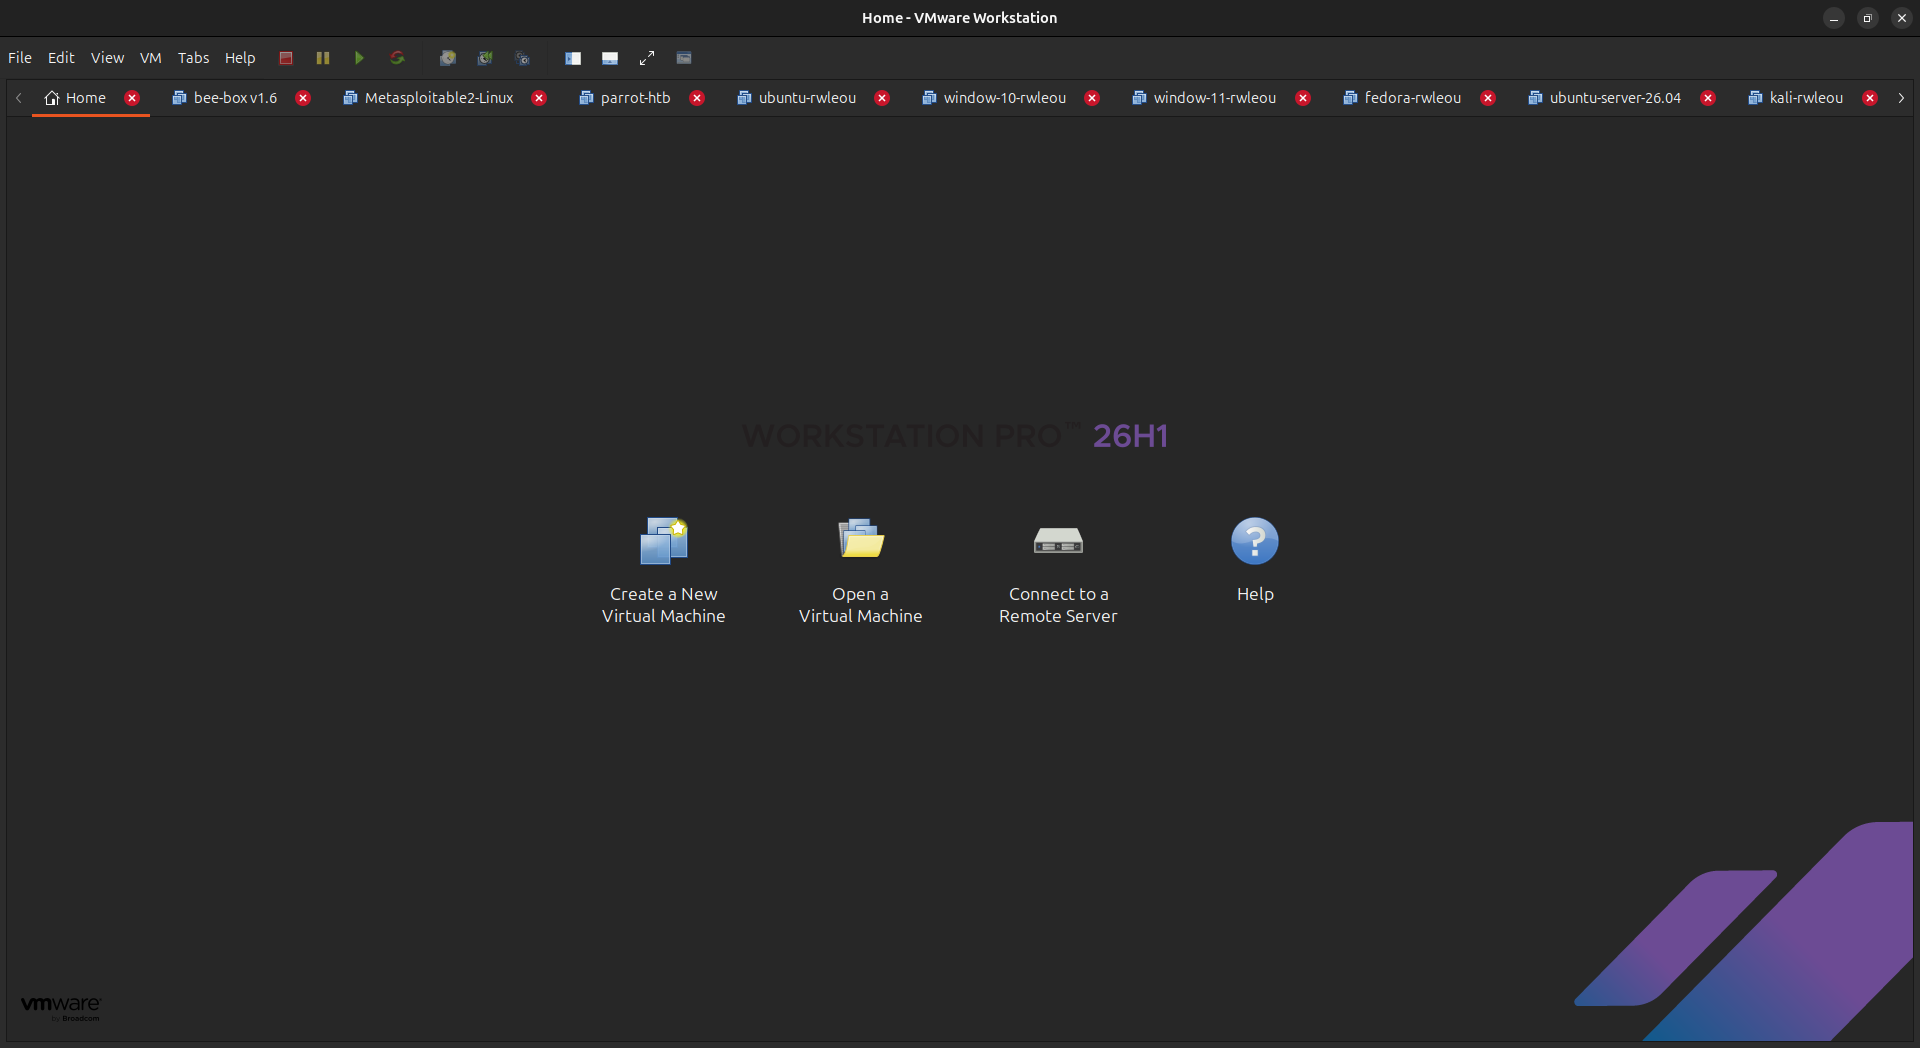
\includegraphics[width=0.9\textwidth]{../src/vmware.png}}
    \caption{VMware Workstation Pro 26H2}
\end{figure}
 \item Now, update and upgrade the newly installed Ubuntu, and install prerequisite packages.
  \begin{lstlisting}[language=bash]
   sudo apt update && sudo apt upgrade -y
   sudo apt install -y git curl openssl\end{lstlisting}
\begin{markdownnote}
\texttt{git} is needed to clone the app repository. \texttt{curl} and \texttt{openssl} are used for Tailscale installation and certificate generation.
\end{markdownnote}
\end{enumerate}

\section{Server Configuration}

\subsection{Assigning Static IP Address}
\indent The VM is configured with a static IP address via Netplan (\texttt{/etc/netplan/50-cloud-init.yaml}) so that services remain reachable after reboots. The VMware NAT network provides connectivity between the host machine and the VM.

\begin{enumerate}
\item Backup \texttt{/etc/netplan/50-cloud-init.yaml} and edit.
\begin{lstlisting}[language=bash]
sudo cp /etc/netplan/50-cloud-init.yaml /etc/netplan/50-cloud-init.yaml.bak
sudo nano /etc/netplan/50-cloud-init.yaml
\end{lstlisting}

\item Now, insert the following configuration.
\begin{lstlisting}[language=bash]
network:
  version: 2
  ethernets:
    ens33:
      dhcp4: false
      addresses:
        - 192.168.10.3/24
      routes:
        - to: default
          via: 192.168.10.2
      nameservers:
        addresses: [8.8.8.8, 8.8.4.4]
\end{lstlisting}

\begin{markdownnote}
\textbf{Note:} Adjust \texttt{ens33}, \textbf{192.168.10.3}, and \textbf{192.168.10.2} to match your VMware network setup. Check your interface name with \texttt{ip a}.
\end{markdownnote}

\item Test and apply:
\begin{lstlisting}[language=bash]
sudo netplan try
sudo netplan apply
ip a
\end{lstlisting}
\end{enumerate}

The server configuration follows a layered approach, addressing networking, security, web serving, and application deployment.

\subsection{Setting up SSH for remote administration}

\begin{enumerate}
\item Install OpenSSH Server (on VM)
\begin{lstlisting}[language=bash]
sudo apt update && sudo apt upgrade -y
sudo apt install openssh-server -y
\end{lstlisting}

\item Verify SSH is Running
\begin{lstlisting}[language=bash]
sudo systemctl status ssh
\end{lstlisting}

\item Connect from Host Machine
Linux/macOS:
\begin{lstlisting}[language=bash]
ssh <username>@192.168.10.3
\end{lstlisting}

Windows (PowerShell):
\begin{lstlisting}[language=bash]
Windows PowerShell
Copyright (C) Microsoft Coporation. All rights reserved.

PS C:\Users\User> ssh <username>@192.168.10.3
\end{lstlisting}

\item Set Up Key-Based Authentication
\begin{itemize}
\item On your host machine, generate an SSH key pair:
\begin{lstlisting}[language=bash]
ssh-keygen -t ed25519 -C "your-email@example.com"
\end{lstlisting}
\item Copy the public key to the VM:
\begin{lstlisting}[language=bash]
ssh-copy-id <username>@192.168.10.3
\end{lstlisting}
\item Test key-based login (should NOT ask for password):
\begin{lstlisting}[language=bash]
ssh <username>@192.168.10.3
\end{lstlisting}
\end{itemize}

\item Disable Password Authentication and Root Login (on VM)
\begin{itemize}
\item Open SSH config:
\begin{lstlisting}[language=bash]
sudo nano /etc/ssh/sshd_config
\end{lstlisting}
\item Find and change these lines:
\begin{lstlisting}[language=bash]
PasswordAuthentication no
PermitRootLogin no
AllowGroups sysadmin dev
\end{lstlisting}
\begin{markdownnote}
\textbf{AllowGroups} restricts SSH login to members of the \texttt{sysadmin} or \texttt{dev} groups only. Other system accounts cannot log in via SSH even if they have valid keys.
\end{markdownnote}
\item Restart SSH:
\begin{lstlisting}[language=bash]
sudo systemctl restart ssh
\end{lstlisting}
\end{itemize}
\begin{markdownnote}
\textbf{Security:} SSH was hardened to allow key-based authentication only. Password authentication and root login were disabled. Only users in the \texttt{sysadmin} or \texttt{dev} groups can log in.
\end{markdownnote}
\end{enumerate}

\subsection{Tailscale Setup (Admin Access)}
Tailscale provides a secure tunnel between your host machine and the VM for administration purposes only. Production traffic does not go through Tailscale.

\begin{enumerate}
\item Install Tailscale on VM
\begin{lstlisting}[language=bash]
curl -fsSL https://tailscale.com/install.sh | sh
sudo tailscale up
\end{lstlisting}

\begin{markdownnote}
Follow the authentication URL to link the VM to your Tailscale account.
\end{markdownnote}

\item Install Tailscale on Host Machine
Download and install from \href{https://tailscale.com/download}{tailscale.com/download}. Sign in with the same account.
\item Verify Tunnel
\begin{itemize}
\item On host, check Tailscale status:
\begin{lstlisting}[language=bash]
tailscale status
\end{lstlisting}
\item Ping the VM via Tailscale:
\begin{lstlisting}[language=bash]
ping <tailscale-ip>
\end{lstlisting}
\item SSH via Tailscale:
\begin{lstlisting}[language=bash]
ssh <username>@<tailscale-ip>
\end{lstlisting}
\end{itemize}
\begin{markdownnote}
\textbf{Note:} Tailscale is used only for sysadmin and dev configuration. The website is accessed via the VM's static IP directly.
\end{markdownnote}
\end{enumerate}

\subsection{User and Group Management}

Two groups were created with distinct privilege levels:

\begin{table}[H]
\centering
\begin{tabularx}{\textwidth}{l l X}
\toprule
\textbf{Group} & \textbf{Privilege} & \textbf{Members} \\
\midrule
sysadmin & Full sudo access & mgkhant, agmyintmyatag, gonyaungwin, agkhantkyaw, santhiritun \\
dev      & Deployment only (no sudo) & kghtutthaw, hanlinhtun, shoonlaeaung, agmyintmyat \\
\bottomrule
\end{tabularx}
\caption{User groups and their privileges}
\end{table}

\begin{markdownnote}
The deployer account (\texttt{agmyintmyat}) owns the web application directory and runs PM2---it never requires sudo access.
\end{markdownnote}

\begin{enumerate}
\item Create Groups
\begin{lstlisting}[language=bash]
sudo groupadd sysadmin
sudo groupadd dev
\end{lstlisting}

\item Create Admin Users
\begin{lstlisting}[language=bash]
sudo useradd -m -s /bin/bash -G sysadmin mgkhant
sudo useradd -m -s /bin/bash -G sysadmin agmyintmyatag
sudo useradd -m -s /bin/bash -G sysadmin gonyaungwin
sudo useradd -m -s /bin/bash -G sysadmin agkhantkyaw
sudo useradd -m -s /bin/bash -G sysadmin santhiritun
\end{lstlisting}

\item Create Developer Users
\begin{lstlisting}[language=bash]
sudo useradd -m -s /bin/bash -G dev kghtutthaw
sudo useradd -m -s /bin/bash -G dev hanlinhtun
sudo useradd -m -s /bin/bash -G dev shoonlaeaung
sudo useradd -m -s /bin/bash -G dev agmyintmyat
\end{lstlisting}

\item Set Passwords
\begin{lstlisting}[language=bash]
sudo passwd mgkhant
sudo passwd agmyintmyatag
sudo passwd gonyaungwin
sudo passwd agkhantkyaw
sudo passwd santhiritun
sudo passwd kghtutthaw
sudo passwd hanlinhtun
sudo passwd shoonlaeaung
sudo passwd agmyintmyat
\end{lstlisting}

\begin{markdownnote}
\textbf{Note:} For project demos on the isolated lab VM, \texttt{12345678} is used as the shared password — never reuse it outside the lab.
\end{markdownnote}

\item Grant sudo to sysadmin group
\begin{lstlisting}[language=bash]
sudo usermod -aG sudo mgkhant
sudo usermod -aG sudo agmyintmyatag
sudo usermod -aG sudo gonyaungwin
sudo usermod -aG sudo agkhantkyaw
sudo usermod -aG sudo santhiritun
\end{lstlisting}

\item Grant sudo to deployer user
\begin{lstlisting}[language=bash]
sudo usermod -aG sudo agmyintmyat
\end{lstlisting}

\item Verify Groups
\begin{lstlisting}[language=bash]
groups mgkhant
groups agmyintmyat
\end{lstlisting}

\item Lock Unused Default Accounts (Optional)
\begin{lstlisting}[language=bash]
sudo usermod -L <unused-default-user>
\end{lstlisting}
\end{enumerate}

\subsection{File and Directory Permissions}
\begin{enumerate}
\item Create Web Directory
\begin{lstlisting}[language=bash]
sudo mkdir -p /var/www/app
\end{lstlisting}

\item Set Ownership
\begin{lstlisting}[language=bash]
sudo chown -R agmyintmyat:dev /var/www/app
\end{lstlisting}

\item Set Permissions
\begin{lstlisting}[language=bash]
sudo chmod 775 /var/www/app
sudo chmod -R 664 /var/www/app/*
\end{lstlisting}

\item Verify Permissions
\begin{lstlisting}[language=bash]
ls -la /var/www/app/
\end{lstlisting}

\item Protect Sensitive Files (if applicable)
\begin{lstlisting}[language=bash]
sudo chown agmyintmyat:dev /var/www/app/.env
sudo chmod 600 /var/www/app/.env
\end{lstlisting}
\begin{markdownnote}
If the application uses a \texttt{.env} file (e.g., for API keys or secrets), restrict it to the owner. The \texttt{lfs-101-notes} app is a static export and does not use a \texttt{.env} file at runtime --- this step only applies if your app requires one.
\end{markdownnote}
\end{enumerate}

\subsection{Apache2 Installation and Configuration}

\begin{enumerate}
\item Install Apache2
\begin{lstlisting}[language=bash]
sudo apt install apache2 -y
\end{lstlisting}

\item Enable Required Modules
\begin{lstlisting}[language=bash]
sudo a2enmod proxy
sudo a2enmod proxy_http
sudo a2enmod rewrite
sudo a2enmod headers
sudo a2enmod ssl
\end{lstlisting}

\item Generate a Self-Signed Certificate
\begin{markdownnote}
Access is via the VM IP address only, and Let's Encrypt cannot issue certificates for bare IPs — so a self-signed certificate is used by default. Browsers will show a one-time trust warning; this is expected.
\end{markdownnote} 
\begin{lstlisting}[language=bash]
sudo openssl req -x509 -nodes -days 365 \
    -newkey ec -pkeyopt ec_paramgen_curve:prime256v1 \
    -keyout /etc/ssl/private/selfsigned.key \
    -out /etc/ssl/certs/selfsigned.crt \
    -subj "/CN=192.168.10.3"
\end{lstlisting}
\item Create Virtual Host Configuration
\begin{lstlisting}[language=bash]
sudo nano /etc/apache2/sites-available/app.conf
\end{lstlisting}
Add the following:
\begin{lstlisting}[language=bash]
<VirtualHost *:80>
    ServerName 192.168.10.3

    # Redirect all HTTP to HTTPS
    RewriteEngine On
    RewriteCond %{HTTPS} off
    RewriteRule ^ https://%{HTTP_HOST}%{REQUEST_URI} [L,R=301]
</VirtualHost>

<VirtualHost *:443>
    ServerName 192.168.10.3

    # SSL Configuration (self-signed certificate generated above)
    SSLEngine on
    SSLCertificateFile /etc/ssl/certs/selfsigned.crt
    SSLCertificateKeyFile /etc/ssl/private/selfsigned.key

    # Security headers (requires mod_headers)
    Header always set Strict-Transport-Security "max-age=63072000; includeSubDomains"
    Header always set X-Content-Type-Options "nosniff"
    Header always set X-Frame-Options "SAMEORIGIN"

    # Health check - served directly by Apache, bypasses Node.js
    ProxyPass /health !
    Alias /health /var/www/app/out/health.html

    # Static assets served directly by Apache (bypass Node.js)
    ProxyPass /_next/static/ !
    Alias /_next/static/ /var/www/app/out/_next/static/

    # Reverse proxy to Next.js
    ProxyPreserveHost On
    ProxyPass / http://127.0.0.1:3000/
    ProxyPassReverse / http://127.0.0.1:3000/

    # Logs
    ErrorLog ${APACHE_LOG_DIR}/app-error.log
    CustomLog ${APACHE_LOG_DIR}/app-access.log combined
</VirtualHost>
\end{lstlisting}
\begin{markdownnote}
The virtual host configuration (\texttt{/etc/apache2/sites-available/app.conf}) defines two blocks: an HTTP-to-HTTPS redirect on port 80, and a full reverse proxy on port 443 with TLS termination. Static assets (\texttt{\_next/static/}) and the health check endpoint are served directly by Apache, bypassing Node.js entirely:
\end{markdownnote}

\item Enable the site
\begin{lstlisting}[language=bash]
sudo a2ensite app.conf
sudo a2dissite 000-default.conf
\end{lstlisting}

\item Hide Server Version (Global Config)
Verify these values in 

\texttt{/etc/apache2/conf-available/security.conf}:
\begin{lstlisting}[language=bash]
ServerTokens Prod
ServerSignature Off
\end{lstlisting}

\item Test and Restart
\begin{lstlisting}[language=bash]
sudo apache2ctl configtest
sudo systemctl restart apache2
sudo systemctl enable apache2
\end{lstlisting}
\end{enumerate}

\subsection{Node.js and Next.js Setup}

\begin{enumerate}
\item Install Node.js (System-Wide via NodeSource)
\begin{lstlisting}[language=bash]
curl -fsSL https://deb.nodesource.com/setup_lts.x | sudo -E bash -
sudo apt install -y nodejs
\end{lstlisting}

\item Verify:
\begin{lstlisting}[language=bash]
node -v
npm -v
\end{lstlisting}

\item Install PM2
PM2 is a process manager for Node.js that handles auto-restarts, log rotation, and startup on boot.
\begin{lstlisting}[language=bash]
sudo npm install -g pm2
\end{lstlisting}
\begin{markdownnote}
\textbf{Important:} Install PM2 as root (with \texttt{sudo}) \textbf{before} switching to the deployer user in the next step. A global install ensures PM2 is available in all users' PATH.
\end{markdownnote}

\item Deploy the Next.js App
\item Login with the developer user:
\begin{lstlisting}[language=bash]
ssh agmyintmyat@<tailscale-ip>
\end{lstlisting}
\item Clone the project
\begin{lstlisting}[language=bash]
cd /var/www
git clone https://github.com/ammdevl/lfs-101-notes.git app
cd app
\end{lstlisting}
\item Install dependencies and build (from the repo root \texttt{/var/www/app}):
\begin{lstlisting}[language=bash]
npm install
npm run build
\end{lstlisting}

\item Start the app with PM2 (from the repo root \texttt{/var/www/app}):
\begin{lstlisting}[language=bash]
npm install -g serve
pm2 start serve --name "nextjs" -- /var/www/app/out
\end{lstlisting}
\begin{markdownnote}
Installing \texttt{serve} globally and running it directly avoids the overhead of \texttt{npx} downloading the package on every cold start.
\end{markdownnote}
\item Save PM2 process list and get the startup command:
\begin{lstlisting}[language=bash]
pm2 save
pm2 startup
\end{lstlisting}
\begin{markdownnote}
PM2 prints a \texttt{sudo env PATH=...} command. Just copy and paste it to enable PM2 to start on boot.
\end{markdownnote}
\item Exit back and login with sysadmin.
\newpage

\item Verify PM2
\begin{lstlisting}[language=bash]
pm2 status
pm2 logs nextjs
curl -I http://127.0.0.1:3000
\end{lstlisting}
\begin{markdownnote}
\textbf{Note:} The app runs from the repo root \texttt{/var/www/app} — all npm commands (install, build, start) are executed in this directory. Verify \texttt{curl -I http://127.0.0.1:3000} returns 200 before troubleshooting Apache; a 503 from Apache means this backend is down.
\end{markdownnote}

\item PM2 Useful Commands
\begin{lstlisting}[language=bash]
pm2 restart nextjs          # restart the app
pm2 stop nextjs             # stop the app
pm2 delete nextjs           # remove the app
pm2 logs nextjs             # view logs
pm2 monit                   # real-time monitoring dashboard
\end{lstlisting}

\end{enumerate}

\subsection{Setting up Firewall (UFW)}
\begin{enumerate}
\item Install and Enable
\begin{lstlisting}[language=bash]
sudo apt install ufw -y
\end{lstlisting}

\item Set rules
\begin{lstlisting}[language=bash]
sudo ufw default deny incoming
sudo ufw default allow outgoing
sudo ufw allow ssh
sudo ufw allow 80/tcp
sudo ufw allow 443/tcp
\end{lstlisting}

\item Enable Firewalls
\begin{lstlisting}[language=bash]
sudo ufw enable
\end{lstlisting}

\item Verify
\begin{lstlisting}[language=bash]
sudo ufw status verbose
\end{lstlisting}
\begin{markdownnote}
\textbf{Important:} Only SSH, HTTP and HTTPS traffic is allowed. All other ports are blocked by default.
\end{markdownnote}

\end{enumerate}
\newpage

\subsection{Setting up Fail2ban}

Fail2ban monitors SSH and Apache authentication logs, automatically banning IPs after 5 failed attempts for 1 hour:

\begin{enumerate}
\item Install
\begin{lstlisting}[language=bash]
sudo apt install fail2ban -y
\end{lstlisting}

\item Configure
add:
\begin{lstlisting}[language=bash]
[DEFAULT]
bantime = 3600
findtime = 600
maxretry = 5

[sshd]
enabled = true
port = ssh
logpath = /var/log/auth.log

[apache-auth]
enabled = true
port = http,https
logpath = /var/log/apache2/app-error.log
\end{lstlisting}

\item Start and Enable
\begin{lstlisting}[language=bash]
sudo systemctl start fail2ban
sudo systemctl enable fail2ban
\end{lstlisting}

\item Verify
\begin{lstlisting}[language=bash]
sudo fail2ban-client status
sudo fail2ban-client status sshd
\end{lstlisting}
\end{enumerate}

\subsection{Automated Backups}
Configure automated daily backups of server configs, SSL certs, and app source:

\begin{lstlisting}[language=bash]
sudo tee /usr/local/bin/backup-server.sh > /dev/null <<'EOF'
#!/usr/bin/env bash
set -euo pipefail
BACKUP_DIR="/var/backups/server"
DATE=$(date +%Y-%m-%d)
KEEP_DAYS=30
mkdir -p "$BACKUP_DIR"
tar czf "$BACKUP_DIR/apache-config-$DATE.tar.gz" \
    /etc/apache2/sites-available/ /etc/apache2/conf-available/ \
    /etc/logrotate.d/apache2-app 2>/dev/null
tar czf "$BACKUP_DIR/ssl-certs-$DATE.tar.gz" \
    /etc/ssl/certs/selfsigned.crt /etc/ssl/private/selfsigned.key 2>/dev/null
cp /etc/ssh/sshd_config "$BACKUP_DIR/ssh-hardening-$DATE.conf" 2>/dev/null || true
cp /etc/fail2ban/jail.local "$BACKUP_DIR/fail2ban-jail-$DATE.local" 2>/dev/null || true
sudo -H -u agmyintmyat pm2 save --force 2>/dev/null || true
cp /home/agmyintmyat/.pm2/dump.pm2 "$BACKUP_DIR/pm2-dump-$DATE.json" 2>/dev/null || true
if [[ -d /var/www/app/.git ]]; then
    tar czf "$BACKUP_DIR/app-source-$DATE.tar.gz" \
        --exclude='node_modules' --exclude='.next' \
        -C /var/www app 2>/dev/null
fi
find "$BACKUP_DIR" -name "*.tar.gz" -mtime +$KEEP_DAYS -delete 2>/dev/null || true
find "$BACKUP_DIR" -name "*.conf" -mtime +$KEEP_DAYS -delete 2>/dev/null || true
find "$BACKUP_DIR" -name "*.local" -mtime +$KEEP_DAYS -delete 2>/dev/null || true
find "$BACKUP_DIR" -name "*.json" -mtime +$KEEP_DAYS -delete 2>/dev/null || true
EOF
sudo chmod +x /usr/local/bin/backup-server.sh
\end{lstlisting}

Schedule daily execution:

\begin{lstlisting}[language=bash]
echo '37 2 * * * root /usr/local/bin/backup-server.sh >> /var/log/server-backup.log 2>&1' | \
    sudo tee /etc/cron.d/server-backup
\end{lstlisting}

Run the initial backup:

\begin{lstlisting}[language=bash]
sudo /usr/local/bin/backup-server.sh
ls -la /var/backups/server/
\end{lstlisting}

\subsection{Verification}
Run these checks to confirm everything works:

\textbf{Services:}
\begin{lstlisting}[language=bash]
sudo systemctl status apache2
sudo systemctl is-active fail2ban
sudo -H -u agmyintmyat pm2 status
\end{lstlisting}

\textbf{HTTP to HTTPS redirect:}
\begin{lstlisting}[language=bash]
curl -I http://192.168.10.3
# Should return: HTTP/1.1 301 Moved Permanently
#                Location: https://192.168.10.3/
\end{lstlisting}

\textbf{HTTPS serving:}
\begin{lstlisting}[language=bash]
curl -skI https://192.168.10.3
# Should return: HTTP/1.1 200 OK
\end{lstlisting}

\textbf{Server version hidden:}
\begin{lstlisting}[language=bash]
curl -skI https://192.168.10.3 | grep -i server
# Should return: Server: Apache (no version number)
\end{lstlisting}

\textbf{File permissions:}
\begin{lstlisting}[language=bash]
ls -la /var/www/app/
# Expected: drwxrwxr-x agmyintmyat dev
\end{lstlisting}

\textbf{Firewall:}
\begin{lstlisting}[language=bash]
sudo ufw status verbose
# Status: active, only 22/tcp, 80/tcp, 443/tcp allowed
\end{lstlisting}

\textbf{Fail2ban:}
\begin{lstlisting}[language=bash]
sudo fail2ban-client status
sudo fail2ban-client status sshd
\end{lstlisting}

\textbf{Boot persistence:}
\begin{lstlisting}[language=bash]
sudo systemctl is-enabled apache2    # should return: enabled
sudo systemctl is-enabled fail2ban   # should return: enabled
sudo systemctl is-enabled pm2-agmyintmyat  # should return: enabled
\end{lstlisting}

\vspace{1.0cm}
Now, on your host machine, open a browser and enter \texttt{192.168.10.3} in address bar, then you will see:

\begin{figure}[h]
    \centering
    \fbox{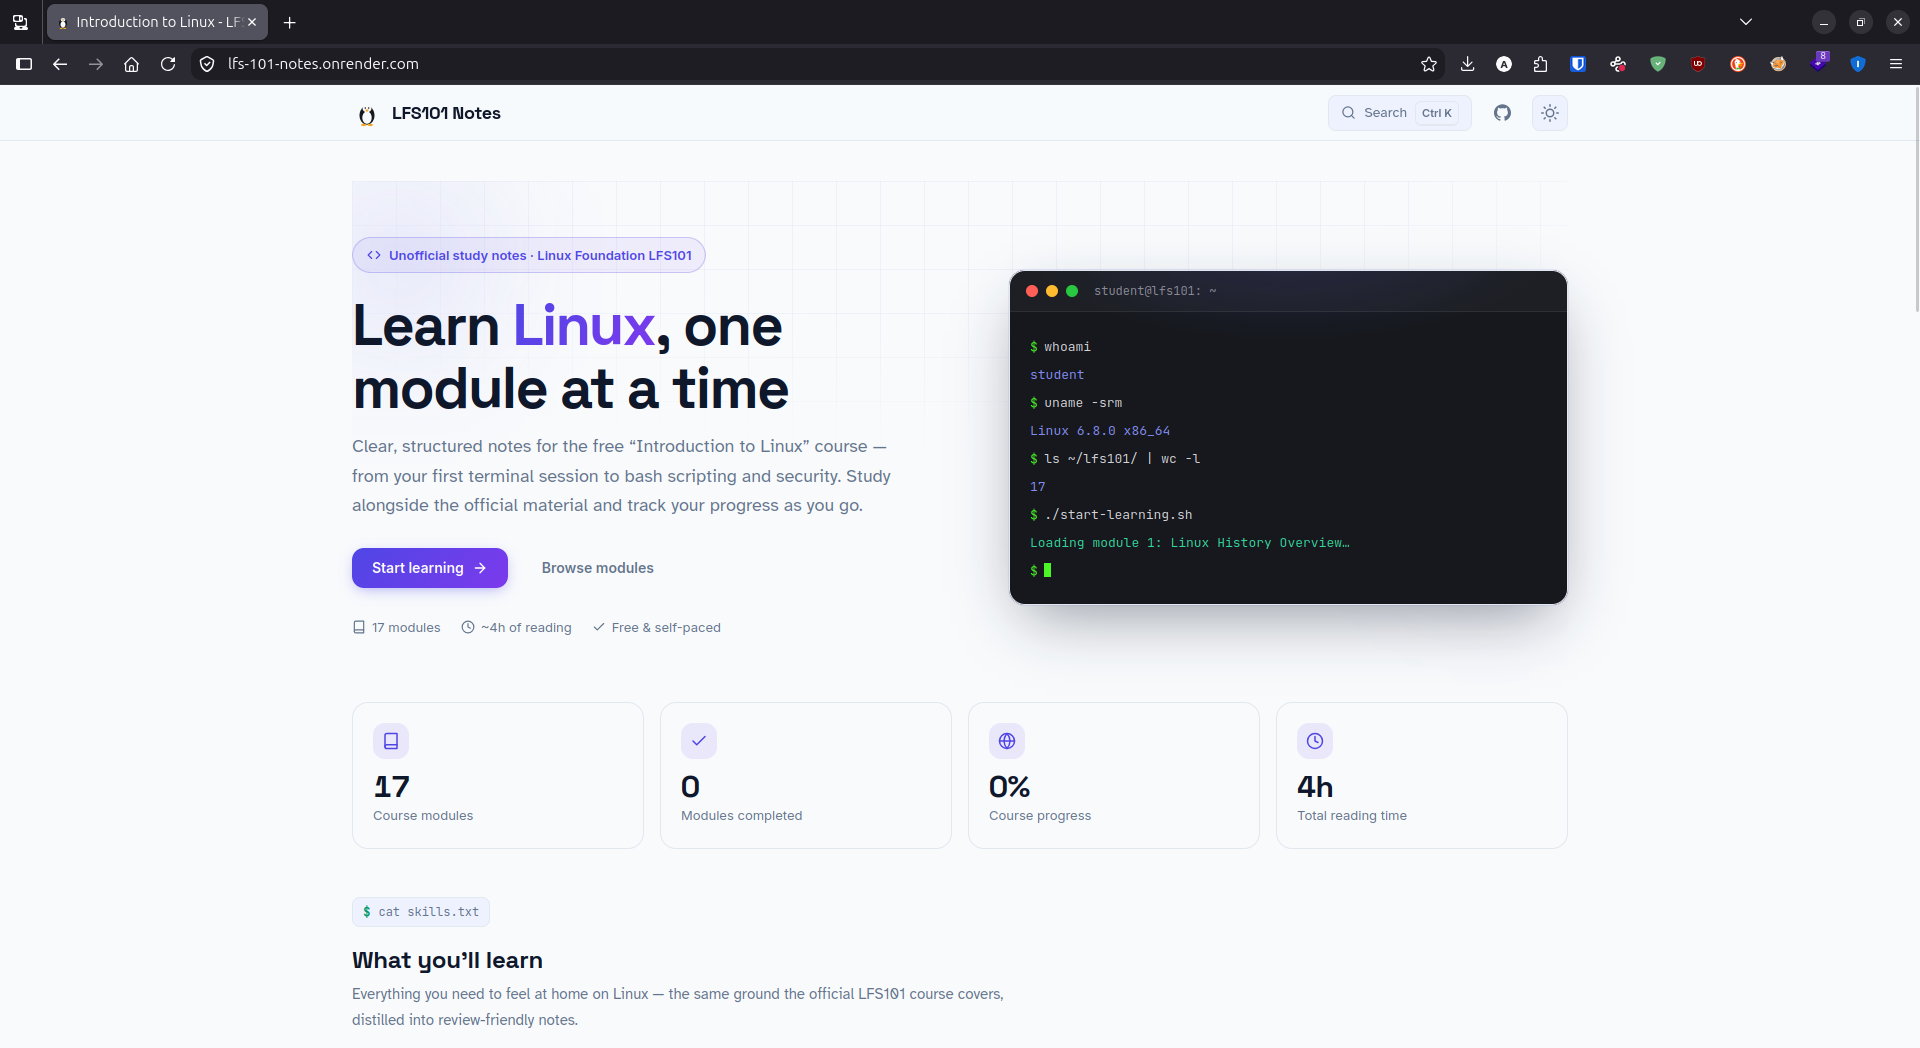
\includegraphics[width=0.9\textwidth]{../src/verification.png}}
    \caption{Verification on client browser}
\end{figure}

\newpage

\chapter{Conclusion}

\section{Conclusion}

\indent This project demonstrates the practical application of Linux system administration concepts in a real-world web server deployment. By setting up Apache2 as a reverse proxy on a VMware Ubuntu 24.04 LTS virtual machine, the team applied user and group management, file permission enforcement, SSH hardening, firewall configuration, intrusion prevention, and TLS encryption.

Key outcomes of the project include:

\begin{itemize}[leftmargin=2em]
    \item A fully functional web server hosting a Next.js application, accessible via HTTPS on the VM's IP address.
    \item Least-privilege access control: the web server process, the deployer account, and administrative users each have distinct, restricted permission levels.
    \item Defense in depth: UFW blocks unauthorized ports, fail2ban prevents brute-force attacks, SSH is hardened to key-only authentication, and Apache's server version information is hidden.
    \item An automated deployment script (\texttt{server-setup.sh}) that reproduces the entire setup, reducing human error and enabling consistent deployments.
    \item Comprehensive documentation including architecture diagrams, troubleshooting guides, and a version-controlled specification.
\end{itemize}

The project reinforced the importance of proper Linux administration practices. Running services as root, using wide-open file permissions, or leaving default configurations in place would have created significant security vulnerabilities. By contrast, the layered approach implemented here---separate accounts, restrictive permissions, firewall, intrusion prevention, and encryption---follows industry best practices for securing web infrastructure.
\vspace{1.0cm}

To get a copy of our project:
\begin{lstlisting}[language=bash]
# Clone github repository
git clone https://github.com/ammdevl/linux-sysadmin-web-server-project

# Navigate to linux-sysadmin-web-server-project/ directory
cd linux-sysadmin-web-server-project/

# Now follow README.md
\end{lstlisting}
\newpage

\section{References}

\paragraph{• Ubuntu Server Guide}
\begin{itemize}[leftmargin=2em]
    \item \url{https://ubuntu.com/server/docs}
\end{itemize}

\paragraph{• Apache2 Documentation}
\begin{itemize}[leftmargin=2em]
    \item \url{https://httpd.apache.org/docs/2.4/}
\end{itemize}

\paragraph{• Apache mod\_proxy Documentation}
\begin{itemize}[leftmargin=2em]
    \item \url{https://httpd.apache.org/docs/2.4/mod/mod_proxy.html}
\end{itemize}

\paragraph{• Next.js Deployment Guide}
\begin{itemize}[leftmargin=2em]
    \item \url{https://nextjs.org/docs/deploying}
\end{itemize}

\paragraph{• Ubuntu UFW Guide}
\begin{itemize}[leftmargin=2em]
    \item \url{https://help.ubuntu.com/community/UFW}
\end{itemize}

\paragraph{• Fail2ban Documentation}
\begin{itemize}[leftmargin=2em]
    \item \url{https://github.com/fail2ban/fail2ban}
\end{itemize}

\paragraph{• Tailscale Documentation}
\begin{itemize}[leftmargin=2em]
    \item \url{https://tailscale.com/kb/}
\end{itemize}

\paragraph{• PM2 Process Manager}
\begin{itemize}[leftmargin=2em]
    \item \url{https://pm2.keymetrics.io/docs/usage/quick-start/}
\end{itemize}

\paragraph{• Netplan Configuration}
\begin{itemize}[leftmargin=2em]
    \item \url{https://netplan.io/}
\end{itemize}

\paragraph{• Linux File Permissions}
\begin{itemize}[leftmargin=2em]
    \item \url{https://www.linuxfoundation.org/blog/linux-file-permissions}
\end{itemize}

\end{document}
